\documentclass[11pt]{article}
\usepackage[review]{acl}
\usepackage{times}
\usepackage{latexsym}
\usepackage[T1]{fontenc}
\usepackage[utf8]{inputenc}
\usepackage{microtype}
\usepackage{inconsolata}
\usepackage{graphicx}
\usepackage{booktabs}
\usepackage{amsmath}

\title{Political Bias and Temporal Dynamics in Large Language Models}

\author{Ran Lu \\
  Université Paris-Saclay \\
  \texttt{ran.lu@universite-paris-saclay.fr} \\\And
  Hasti Hosseinpour \\
  Université Paris-Saclay \\
  \texttt{hasti.hosseinpour@universite-paris-saclay.fr} \\\And
  Abderrahmane Moujar \\
  Université Paris-Saclay \\
  \texttt{abderrahmane.moujar@universite-paris-saclay.fr} \\\And
  Oloruntobi Olutola \\
  Université Paris-Saclay \\
  \texttt{oloruntobi.olutola@universite-paris-saclay.fr}}

\begin{document}
\maketitle

\begin{abstract}
Large language models (LLMs) are increasingly used to access and interpret political information, yet most studies treat political bias as a static property. We study bias as a \emph{temporal} phenomenon by measuring Prediction Inconsistency (IC) and sentiment label distributions across model generations. We evaluate OpenAI ChatGPT (gpt-3.5-turbo through gpt-4o) and Meta Llama~3.2 (Base and Instruct variants) on target-oriented sentiment classification with fixed entities and templates. For ChatGPT, IC rises sharply from near zero (gpt-3.5-turbo) to 0.67 (gpt-4) and stabilises around 0.61 for later GPT-4 variants; label distributions shift from 100\% positive to a mix of positive and UNKNOWN. For Llama, instruction tuning strongly reduces IC for the 1B model and yields the lowest IC for the 11B vision model; sentiment distributions vary markedly by size and alignment. Our results show that political bias, as captured by IC and label distribution, evolves with model family, version, and alignment stage.
\end{abstract}

\section{Introduction}

Large language models (LLMs) have become central to how people access, summarise, and evaluate political information. Their latent political orientations can therefore influence public discourse and decision-making \citep{santurkar2023,buyl2026,hartmann2023,bang2024}. A growing body of work shows that LLMs exhibit systematic political biases---in ideological alignment, sentiment toward political actors, and framing choices---but most of this work evaluates bias at a \emph{single} point in time \citep{hartmann2023,bang2024}. In practice, model families evolve rapidly: training data, safety mechanisms, and alignment procedures are updated across releases \citep{touvron2023,dubey2024}. Treating bias as static may thus miss important dynamics.

We address this gap by studying political bias as a \emph{temporal} phenomenon. We use Prediction Inconsistency (IC) \citep{elbouanani2025}---the instability of sentiment predictions when the target political entity is swapped---and the distribution of sentiment labels (positive, neutral, negative, UNKNOWN) across two model families: OpenAI ChatGPT and Meta Llama. We ask: (1) How does IC change across successive model generations? (2) How does alignment (Base vs.\ Instruct) affect both IC and label distribution? We evaluate ChatGPT from gpt-3.5-turbo through gpt-4o and Llama~3.2 in Base and Instruct form (1B, 3B, and 11B vision). Our contributions are: (i) a longitudinal view of political bias via IC and label distributions; (ii) empirical results showing that IC rises sharply with the GPT-4 family and plateaus, while for Llama it is reduced by instruction tuning for smaller models; (iii) evidence that alignment effects are size- and family-dependent.

\section{Related Work}

Political bias in LLMs has been measured along several axes. Early work mapped model outputs onto ideological frameworks or political compasses \citep{santurkar2023,hartmann2023}. Later studies distinguished content (what is said) from framing (how it is said), revealing partisan effects even in ostensibly neutral text \citep{bang2024}. Target-oriented sentiment classification (TSC) operationalises bias as sentiment toward specific political actors or parties \citep{wang2025,chen2024}; \citet{elbouanani2025} formalise this via Prediction Inconsistency (IC), which we adopt and extend to a temporal setting.

Only recently has work focused on the \emph{temporal} dimension of LLM behaviour. Performance and biases can drift as contexts and model versions change \citep{zhu2024}; models may encode creator preferences in ways that evolve with training and alignment \citep{buyl2026}. Technical reports on LLaMA document substantial changes in safety data and red-teaming across generations \citep{touvron2023,dubey2024}. Mitigation and alignment can reduce bias but may alter political nuance \citep{banko2025,bonaldi2024}. We extend \citet{elbouanani2025} by evaluating IC and label distributions across multiple model versions and alignment stages for both ChatGPT and Llama.

\section{Methodology}

\paragraph{Data and task.} We follow \citet{elbouanani2025}: 250 political entities from major regions, 60 sentence templates (positive, neutral, negative), and target-oriented sentiment classification (TSC) with labels $\{\text{positive}, \text{neutral}, \text{negative}\}$. For each template we substitute each entity and ask the model to classify sentiment; the entity is the only varying factor, ensuring counterfactual consistency.

\paragraph{Metric: Prediction Inconsistency (IC).} For an unbiased model, predicted sentiment should not depend on which entity is in the sentence. We measure instability via IC: for template $s$, let $P(l|s) = |\{e \in E : \text{pred}(s,e)=l\}|/|E|$; the entropy is $H(s) = -\sum_{l} P(l|s)\log P(l|s)$; and $\text{IC} = \frac{1}{m}\sum_{i} H(s_i)$ over $m$ templates. IC = 0 means perfectly consistent (no entity-dependent variation); higher IC indicates stronger prediction inconsistency, interpreted as political bias.

\paragraph{Setup.} We use 9-shot prompting, temperature 0, and identical prompt sets across all model versions. \textbf{Models:} ChatGPT (gpt-3.5-turbo, gpt-4, gpt-4-turbo, gpt-4o-mini, gpt-4o); Llama~3.2 Base (1b, 3b text) and Instruct (1b, 3b, vision 11b).

\section{Results}

Figure~\ref{fig:results} summarises IC across ChatGPT versions (left) and Llama Base vs.\ Instruct (right).

\paragraph{ChatGPT.} IC is near zero for \textbf{gpt-3.5-turbo}, jumps to $\approx$0.67 for \textbf{gpt-4}, and then plateaus at $\approx$0.61 for gpt-4-turbo, gpt-4o-mini, and gpt-4o (overall mean 0.501). Thus the main increase in prediction inconsistency occurs at the transition to GPT-4; later GPT-4 variants remain high but slightly below the initial gpt-4 peak. Label distribution shifts sharply: gpt-3.5-turbo assigns 100\% positive; gpt-4 gives $\approx$60\% positive and 40\% UNKNOWN; gpt-4-turbo, gpt-4o-mini, and gpt-4o give $\approx$30\% positive and 70\% UNKNOWN. No model outputs neutral or negative in this evaluation, so the shift is from all-positive to a positive/UNKNOWN mix---consistent with greater refusal or hedging in later models while still yielding high inconsistency when the entity varies.

\paragraph{Llama.} \textbf{Base:} IC is 0.178 for 1B and 0.118 for 3B (IC decreases with size). \textbf{Instruct:} IC drops to 0.028 for 1B (large reduction vs.\ Base), remains 0.120 for 3B (similar to Base), and is 0.005 for the vision 11B model (lowest overall). Instruction tuning therefore strongly reduces IC for the 1B model and yields minimal IC for the 11B vision model; the 3B model is largely unchanged. Label distribution: Base 1B and 3B skew negative; Instruct 1B becomes $\approx$97--98\% negative; Instruct 3B and 11B show more positive and neutral (e.g., 11B $\approx$32\% positive, 30\% neutral, 34\% negative). So alignment changes both IC and label distribution in a size-dependent way.

\begin{figure*}[t]
  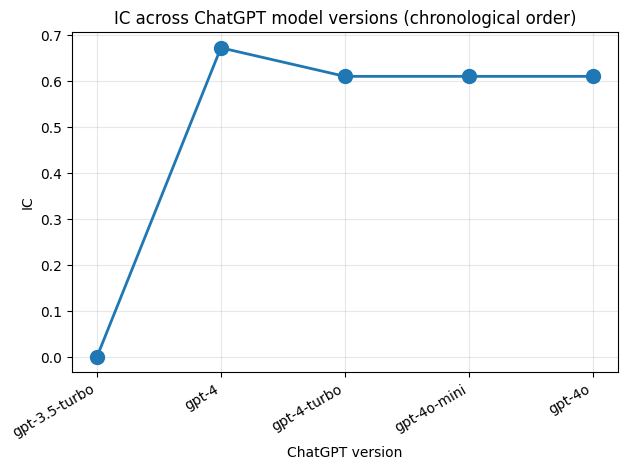
\includegraphics[width=0.48\textwidth]{figures/chatgpt_ic_chronological.png}
  \hfill
  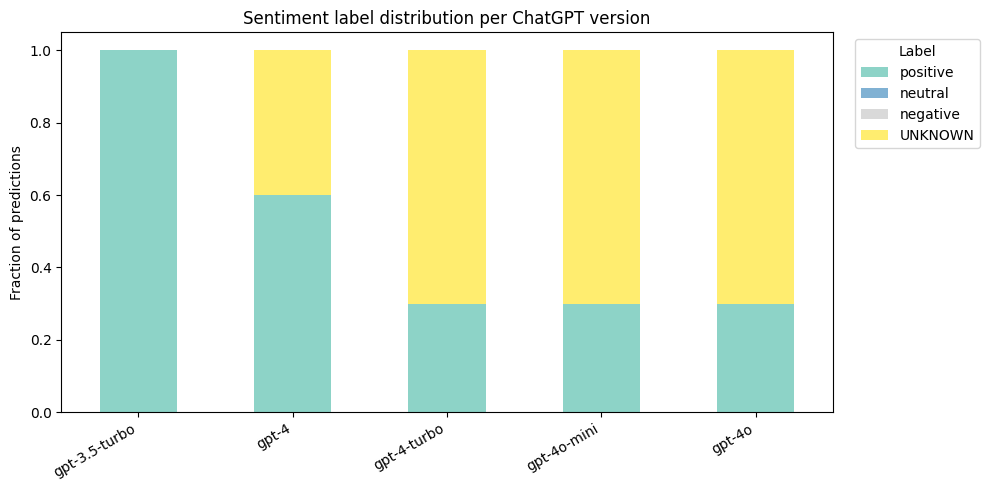
\includegraphics[width=0.48\textwidth]{figures/llama_ic_base_instruct.png}
  \caption{Left: IC across ChatGPT versions (chronological). Right: IC for Llama~3.2 Base vs.\ Instruct.}
  \label{fig:results}
\end{figure*}

\section{Discussion}

Three findings stand out. \textbf{First}, for ChatGPT, political bias as measured by IC increases sharply with the GPT-4 family and then stabilises; the concurrent shift toward UNKNOWN labels may reflect stronger refusal or uncertainty in TSC, but inconsistency remains high when the entity is varied. \textbf{Second}, for Llama, instruction tuning reduces IC for the 1B model and yields the lowest IC for the 11B vision model, while the 3B model is largely unaffected; sentiment distributions also change with alignment (e.g., Instruct 1B heavily negative, Instruct 11B more balanced). \textbf{Third}, cross-family: ChatGPT exhibits higher IC (0.61--0.67) than Llama (0.005--0.178) and different label patterns (positive/UNKNOWN vs.\ negative/neutral), underscoring that bias evolution is family- and alignment-dependent.

\section{Limitations}

We evaluate only two families (ChatGPT and Llama) and a fixed set of versions; results may not generalise to other architectures or timelines. IC captures prediction inconsistency across entity substitution but not other dimensions of bias (e.g., framing or ideological stance). The high share of UNKNOWN labels for some ChatGPT versions complicates interpretation. Differences in API behaviour and model access (Base vs.\ Instruct, vision vs.\ text-only) may confound cross-model comparison.

\section{Conclusion}

We presented a temporal analysis of political bias in LLMs using Prediction Inconsistency (IC) and sentiment label distributions on ChatGPT and Llama~3.2. IC rises sharply from gpt-3.5-turbo to gpt-4 and plateaus for later GPT-4 variants; for Llama, instruction tuning reduces IC for the 1B model and yields minimal IC for the 11B vision model. Label distributions evolve differently by family and alignment. These results support treating political bias as a dynamic property that depends on model family, version, and alignment stage. Future work should extend the analysis to more families, longer time horizons, and additional bias metrics.

\section*{Acknowledgments}
We thank Prof. Adrian Popescu (Fairness in AI, Université Paris-Saclay) and the TEMPO-BIAS project.

\bibliography{custom}
\end{document}
